\documentclass[11pt]{article}
\usepackage[margin=1in]{geometry}
\usepackage{graphicx}
\usepackage{float}
\usepackage{amsmath}
\usepackage{booktabs}
\usepackage{enumitem}
\usepackage[hidelinks]{hyperref}

\setlist{itemsep=2pt, topsep=4pt}
\setlength{\parskip}{4pt}

\title{\textbf{ML-Driven PVT-Variation-Aware Leakage Estimation}\\[4pt]
       \large Digital VLSI Design Project}

\author
{
    Abhinav Venkata Kota \\ Roll No: 2024102059
    \and
    Nikhil Atkuru \\ Roll No: 2024102039
    \and
    Pranav Adarsh \\ Roll No: 2024102028
    \and
    Srikar Durbha \\ Roll No: 2024112010
}

\date{}

\begin{document}

\maketitle
\tableofcontents

\vspace{1em}
\noindent\textbf{Code repository:} \url{https://github.com/DevAbhinav-23/DVD_Project.git}
\newpage

% ==================================================================
\section{Introduction}

Leakage current is a major part of the power used by circuits in modern
technologies, and it changes strongly with process, supply voltage and
temperature (PVT). Running SPICE for every possible condition is slow. In
this project we use SPICE to build transistor datasets for the 22\,nm PTM
model, train machine learning models that predict the leakage currents of a
single transistor, and then use these models to estimate the leakage of
logic gates and of an 8-bit parity checker, comparing the results with SPICE.

% ==================================================================
\section{Setup}

\begin{table}[H]
\centering
\begin{tabular}{ll}
\toprule
Model file & 22nm\_MGK.pm (PTM 22\,nm metal gate, BSIM4) \\
Nominal supply & $V_{DD} = 0.9$\,V \\
Channel length & $L = 22$\,nm \\
Test circuit & 8-bit parity checker: 8 data bits + 1 parity bit (9 inputs) \\
Simulator & ngspice-42 (datasets and gates), ngspice-47 (parity circuit) \\
Software & Python 3.12 \\
\bottomrule
\end{tabular}
\caption{Project setup.}
\label{tab:setup}
\end{table}

Every netlist uses the options line
\begin{center}
\texttt{.options gmin=1e-18 abstol=1e-18 reltol=1e-6 vntol=1e-9}
\end{center}
Every transistor has drain and source areas $AD = AS = W \times 2L$.

% ==================================================================
\section{Data Generation}
\label{sec:data}

\subsection{Datasets}

We made one dataset for each of the four transistor cases: NMOS ON, NMOS OFF,
PMOS ON and PMOS OFF. Each dataset has 10{,}000 rows. Every row stores the
inputs ($V_{DD}$, temperature, $W$, $V_d$, $V_s$, $V_g$, $V_b$, vth0, toxe,
ndep, u0, xj) and the four terminal currents ($I_d$, $I_g$, $I_s$, $I_b$)
found by SPICE. A current is positive when it flows into the transistor.

\subsection{How the samples were drawn}

Each input was picked at random from the ranges in
Table~\ref{tab:ranges}. The gate and body voltages are fixed by the case
(Table~\ref{tab:vgvb}).

\begin{table}[H]
\centering
\begin{minipage}{0.6\textwidth}
\centering
\begin{tabular}{ll}
\toprule
Input & Range \\
\midrule
$V_{DD}$ & 0.81 to 0.99\,V \\
$V_d$, $V_s$ & 0 to $V_{DD}$ \\
Width $W$ & 22 to 176\,nm \\
Temperature & $-40$ to $125\,^\circ$C \\
vth0, toxe, ndep, u0, xj & nominal value $\pm 10\%$ \\
\bottomrule
\end{tabular}
\caption{Ranges of the sampled inputs.}
\label{tab:ranges}
\end{minipage}%
\begin{minipage}{0.38\textwidth}
\centering
\begin{tabular}{lcc}
\toprule
Case & $V_g$ & $V_b$ \\
\midrule
NMOS ON  & $V_{DD}$ & 0 \\
NMOS OFF & 0 & 0 \\
PMOS ON  & 0 & $V_{DD}$ \\
PMOS OFF & $V_{DD}$ & $V_{DD}$ \\
\bottomrule
\end{tabular}
\caption{Gate and body voltages.}
\label{tab:vgvb}
\end{minipage}
\end{table}

\subsection{Netlists and simulation}

For every sample, a Python script writes a small netlist with:
\begin{enumerate}
    \item the NMOS or PMOS model from the model file, with vth0, toxe, ndep,
          u0 and xj replaced by the sample's values;
    \item one transistor with the sample's $W$, and a separate DC voltage
          source on each of its four terminals;
    \item the sample's temperature and an \texttt{.op} (DC operating point)
          analysis.
\end{enumerate}
The current through each source gives the current of that terminal. The
netlists are run in ngspice in groups of 250, and the currents are read
back and saved to the dataset.

\subsection{Data check}

\paragraph{Current sum.}
The four terminal currents of a transistor must add up to zero. We checked
this for every row of every case (Table~\ref{tab:kcl}, Fig.~\ref{fig:kcl}).
A row passes if the leftover sum is below $10^{-3}$ of its largest current
plus $10^{-13}$\,A; every row of all four datasets passes.

\begin{table}[H]
\centering
\begin{tabular}{lcc}
\toprule
Case & Largest $|I_d+I_g+I_s+I_b|$ (A) & Rows passing \\
\midrule
NMOS ON  & $1.6\times10^{-15}$ & 10{,}000 / 10{,}000 \\
NMOS OFF & $2.4\times10^{-21}$ & 10{,}000 / 10{,}000 \\
PMOS ON  & $1.1\times10^{-16}$ & 10{,}000 / 10{,}000 \\
PMOS OFF & $1.1\times10^{-14}$ & 10{,}000 / 10{,}000 \\
\bottomrule
\end{tabular}
\caption{Kirchhoff check for each case.}
\label{tab:kcl}
\end{table}

\paragraph{Ranges.}
No values are missing, and every input lies inside its range.

\paragraph{Trends.}
The currents change with temperature, threshold voltage and oxide thickness
in the expected way (Figs.~\ref{fig:temp}--\ref{fig:toxe}). The PMOS vth0 is
negative ($-0.254$\,V nominal), so for both devices the trend is stated
with the threshold magnitude $|\text{vth0}|$:
\begin{itemize}
    \item OFF current increases with temperature: about $16\times$ (NMOS) and
          $10\times$ (PMOS) from $-40$ to $125\,^\circ$C.
    \item OFF current decreases as $|\text{vth0}|$ increases: about
          $4\times$ (NMOS) and $3\times$ (PMOS) lower over the $\pm 10\%$
          range. For the PMOS this means the OFF current rises as the signed
          vth0 goes from $-0.279$ to $-0.229$\,V.
    \item Gate current decreases as toxe increases: about $10\times$ lower
          over the $\pm 10\%$ range.
\end{itemize}

\begin{figure}[H]
\centering
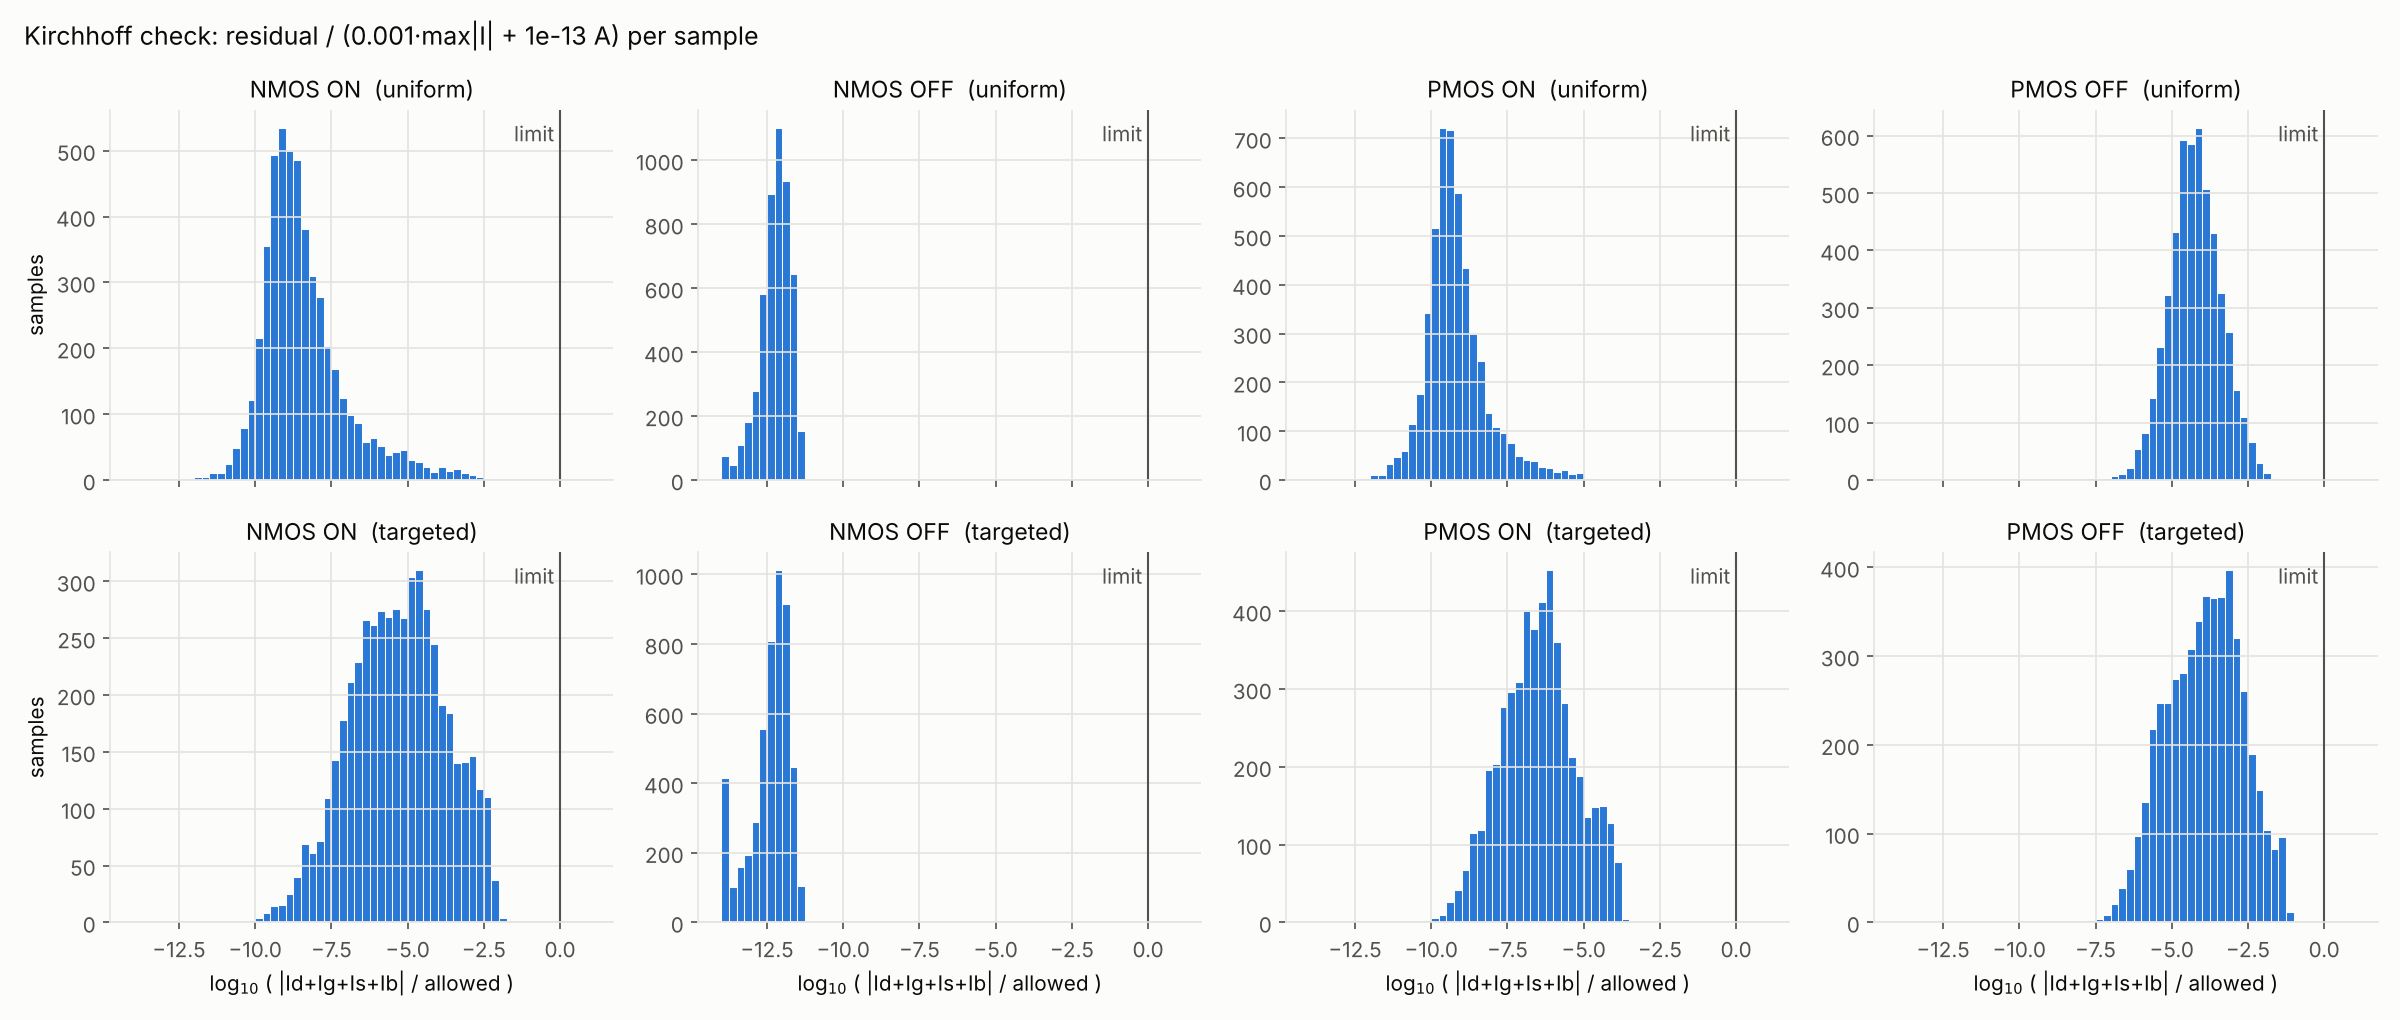
\includegraphics[width=0.6\textwidth]{kcl_check.png}
\caption{Sum of the four terminal currents for every row.}
\label{fig:kcl}
\end{figure}

\begin{figure}[H]
\centering
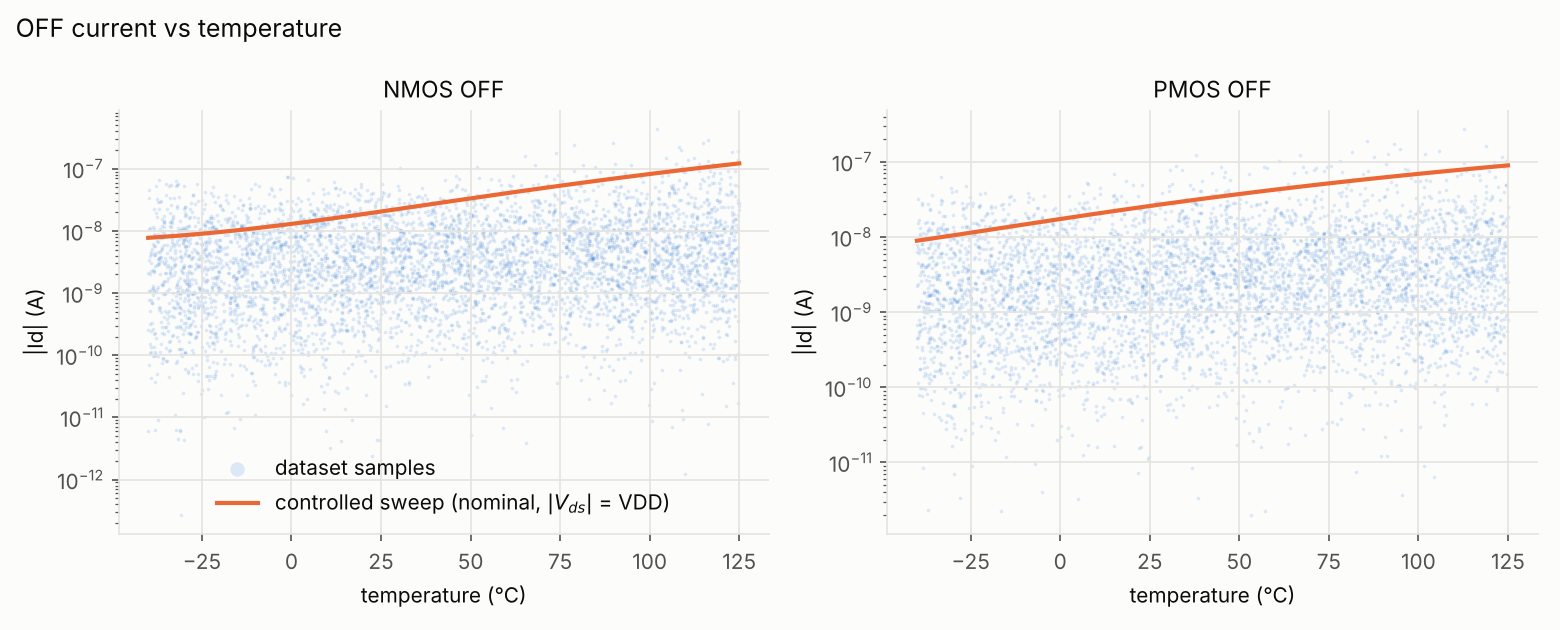
\includegraphics[width=0.6\textwidth]{off_current_vs_temp.png}
\caption{OFF current vs temperature.}
\label{fig:temp}
\end{figure}

\begin{figure}[H]
\centering
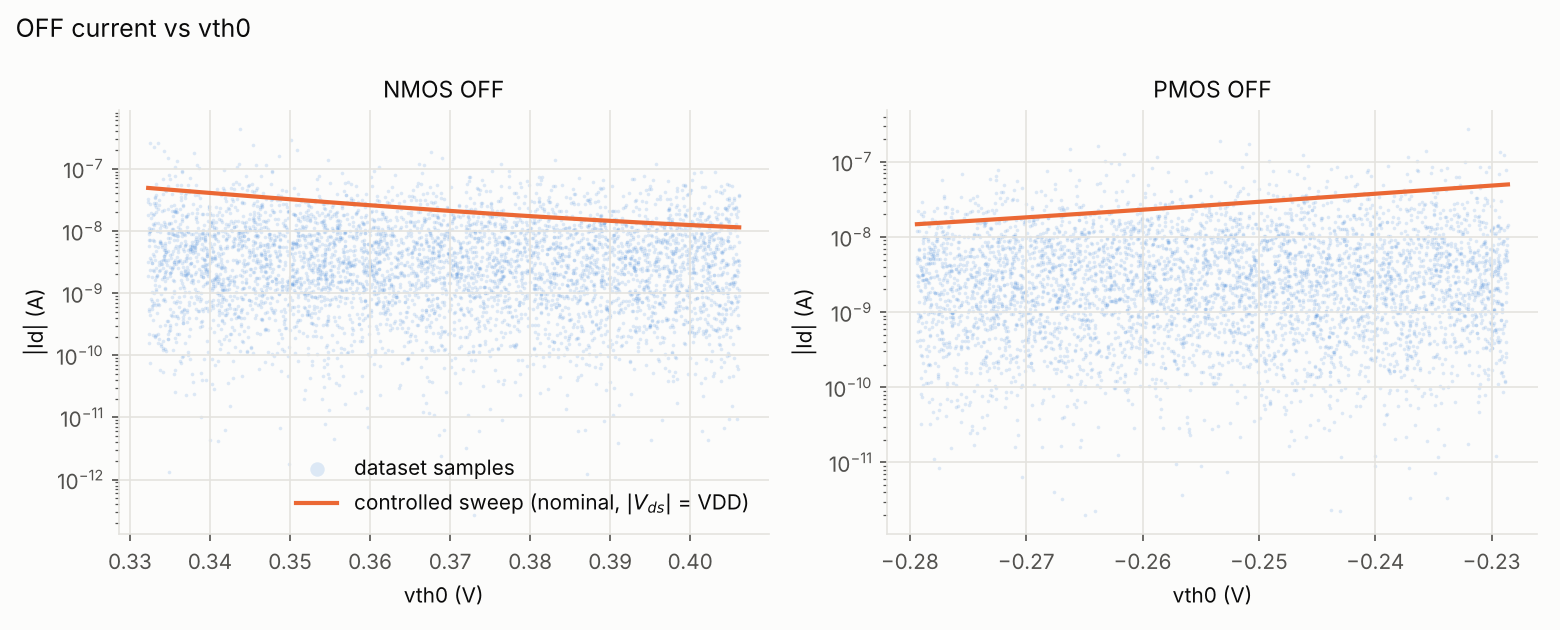
\includegraphics[width=0.6\textwidth]{off_current_vs_vth0.png}
\caption{OFF current vs vth0.}
\label{fig:vth0}
\end{figure}

\begin{figure}[H]
\centering
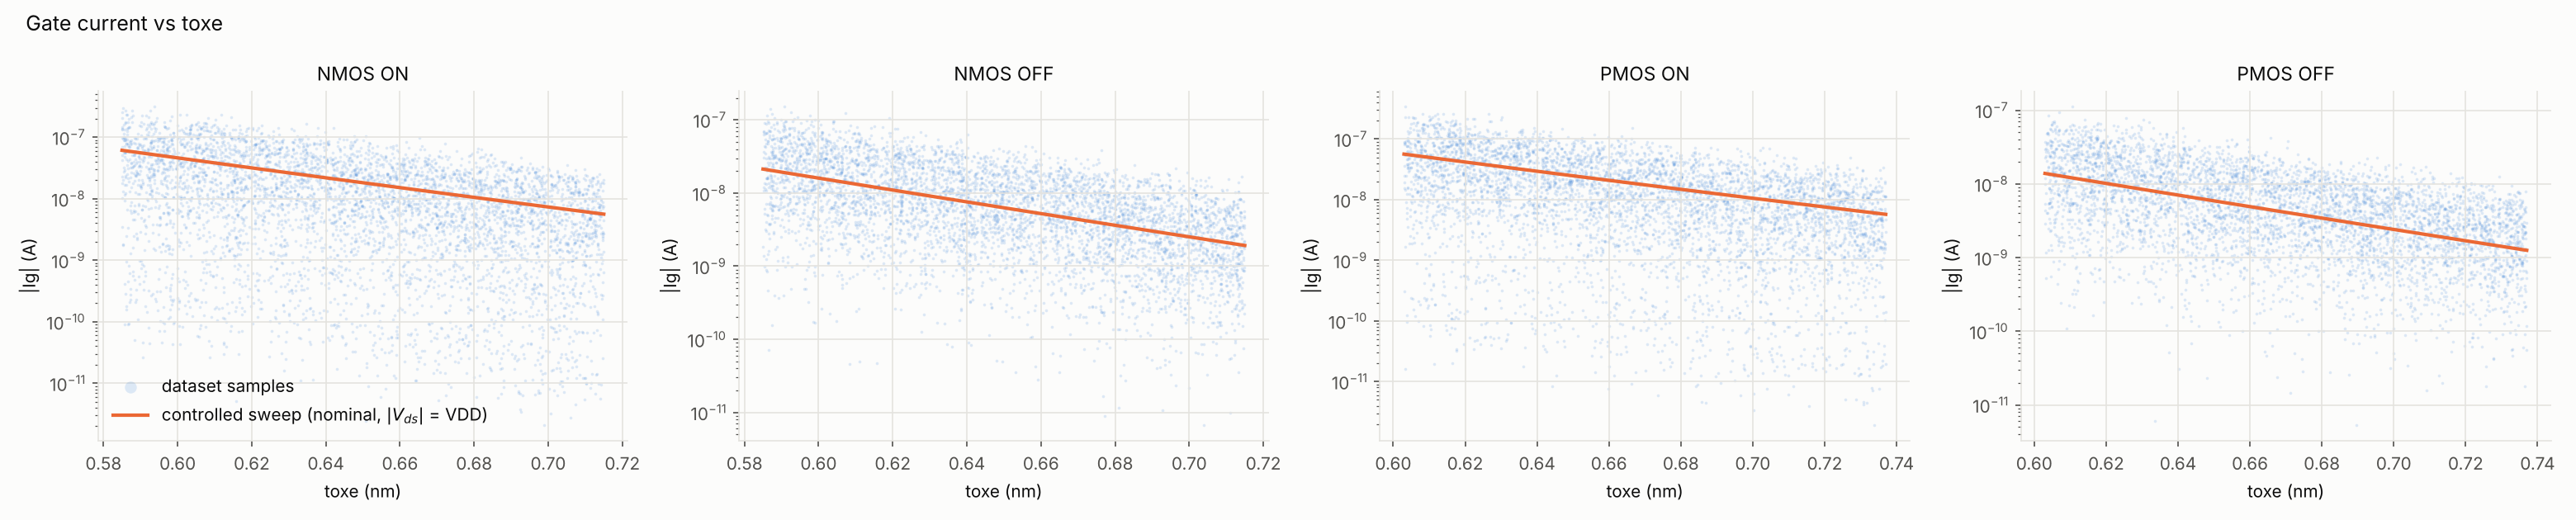
\includegraphics[width=0.9\textwidth]{gate_current_vs_toxe.png}
\caption{Gate current vs toxe.}
\label{fig:toxe}
\end{figure}

% ==================================================================
\section{Transistor-Level ML Models}
\label{sec:models}

\subsection{Data and method}
The models use the four datasets of Section~\ref{sec:data}, 10{,}000 SPICE
rows per case. The 12 inputs predict $I_\mathrm{d}$,
$I_\mathrm{g}$, $I_\mathrm{s}$ and $I_\mathrm{b}$. Data is split 70/15/15
with a fixed seed (42).

Because currents span 15 decades, each model predicts $y=\log_{10}|I|$ and a
LightGBM classifier predicts the sign, so $I=\operatorname{sign}(I)\cdot10^{y}$.
The inputs are extended with physics-based features: voltage differences,
$1/kT$, log process parameters and subthreshold exponents such as
$(V_\mathrm{gs}-|\mathrm{vth0}|)/kT$.

\subsection{Models and selection}
The four families were chosen to span the main kinds of regression model,
from a simple baseline to a flexible neural network, so the comparison shows
how much model complexity the leakage problem needs:
\begin{itemize}
  \item \textbf{Polynomial ridge} (degree 2--3): the baseline. It is fast and
        interpretable and tests whether a smooth fixed functional form of the
        physics features is enough.
  \item \textbf{Random forest} (400 trees): a robust, widely used non-linear
        model that needs no feature scaling and little tuning, giving a
        reference for tree-based methods.
  \item \textbf{LightGBM} (boosted trees, early stopping): usually the most
        accurate model on tabular data such as SPICE sweeps, and fast to train.
  \item \textbf{MLP} (3$\times$64 tanh, L-BFGS): a smooth function
        approximator suited to the continuous, exponential device equations;
        one network predicts all four currents, so they share what it learns
        about the device.
\end{itemize}
For each case the model with the lowest validation score, mean over
terminals of $(\text{median}+\text{p95})/2$ relative error, was chosen.

\begin{table}[H]
\centering\small
\begin{tabular}{lcccc|c}
\toprule
 & \multicolumn{4}{c|}{Validation median / p95 error (\%)} & Test median / \\
Case & Poly ridge & Rand.\ forest & LightGBM & MLP & p95 (\%) \\
\midrule
NMOS ON  & 14.0 / 74 & 13.3 / 68 & 5.8 / 31 & \textbf{2.8 / 29} & 2.8 / 31 \\
NMOS OFF & 19.4 / 99 & 9.1 / 51  & 5.5 / 33 & \textbf{2.8 / 12} & 3.0 / 14 \\
PMOS ON  & 12.4 / 67 & 12.9 / 61 & \textbf{5.4 / 30} & 2.5 / 37 & 5.4 / 31 \\
PMOS OFF & 21.0 / 94 & 9.9 / 52  & 5.5 / 31 & \textbf{2.9 / 13} & 3.0 / 13 \\
\bottomrule
\end{tabular}
\caption{Model comparison (mean of four terminals). Bold: chosen model; the
test column is for the chosen model.}
\label{tab:results}
\end{table}

\begin{table}[H]
\centering\small
\begin{tabular}{lcccc}
\toprule
Case & Poly ridge & Rand.\ forest & LightGBM & MLP \\
\midrule
NMOS ON  & 0.990 & 0.992 & 0.998 & \textbf{0.995} \\
NMOS OFF & 0.918 & 0.982 & 0.991 & \textbf{0.998} \\
PMOS ON  & 0.989 & 0.993 & \textbf{0.997} & 0.988 \\
PMOS OFF & 0.902 & 0.982 & 0.992 & \textbf{0.997} \\
\bottomrule
\end{tabular}
\caption{Validation $R^2$ on $\log_{10}|I|$ (mean of four terminals). Bold:
chosen model.}
\label{tab:r2}
\end{table}

\subsection{Results}
The MLP had the lowest median error in every case and was chosen for NMOS ON,
NMOS OFF and PMOS OFF. For PMOS ON, LightGBM won on the selection score (17.6
vs 19.7) through its better p95, although the MLP's median is lower; the
rule's choice was kept. All four families reach a high $R^2$ on
$\log_{10}|I|$ (Table~\ref{tab:r2}); the polynomial model is weakest on the
OFF cases, mainly on the body current. On the test set the chosen models
reach 2.8--3.0\% median error (5.4\% for PMOS ON), with $R^2 \ge 0.98$ and
the correct sign in 98--100\% of rows (Table~\ref{tab:results},
Fig.~\ref{fig:parity}). The largest
errors are the OFF body current (junction leakage) and the ON-device
$I_\mathrm{d}, I_\mathrm{s}$ at $V_\mathrm{ds}\approx0$, which the gate
formula does not use.

Used in Sections~\ref{sec:gates} and~\ref{sec:circuit}, the models give
\textbf{1.33\% median error (98.2\% mean accuracy)} over 3{,}600 gate
simulations and \textbf{1.14\% median (98.6\% mean accuracy)} over 102{,}400
simulations of the 9-input parity checker. The learning curve
(Fig.~\ref{fig:learning}) shows the OFF and PMOS ON models still improving at
7k training rows, so more training data or an MLP ensemble would improve
them further.

\begin{figure}[H]
\centering
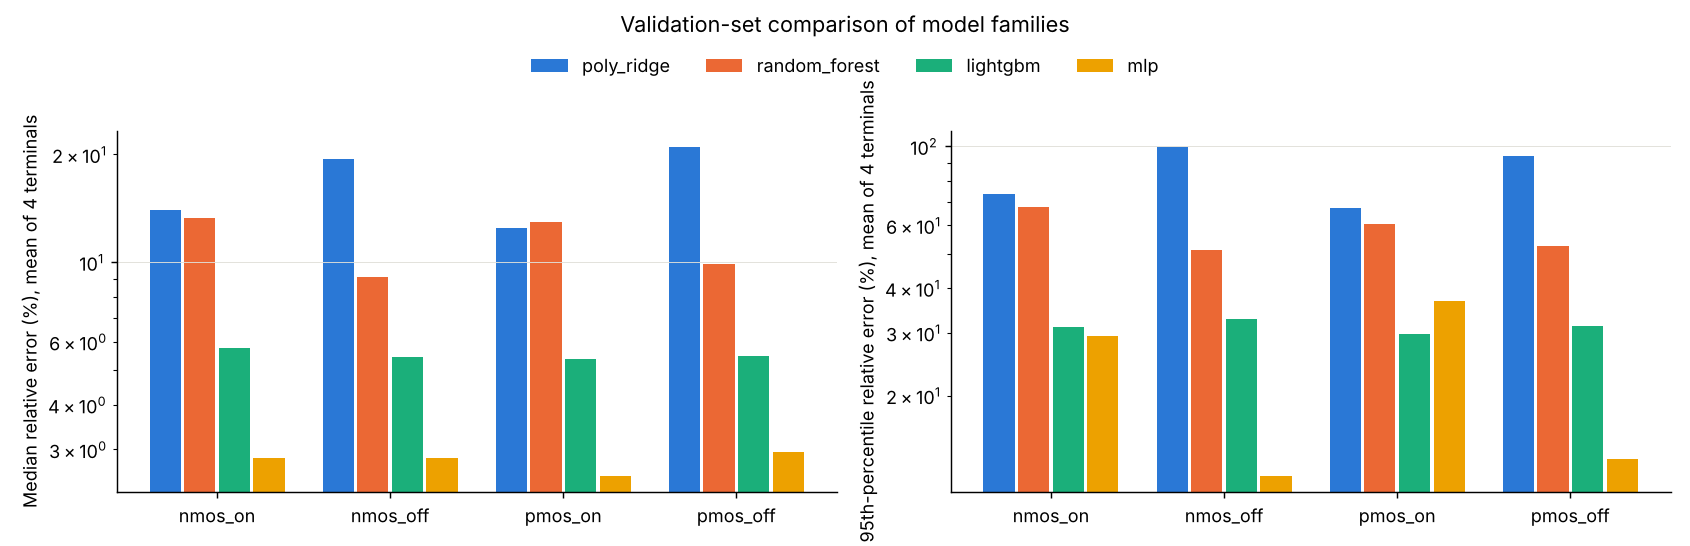
\includegraphics[width=0.85\linewidth]{family_comparison.png}
\caption{Validation error of the four model families per case: median (left)
and p95 (right).}
\label{fig:family}
\end{figure}

\begin{figure}[H]
\centering
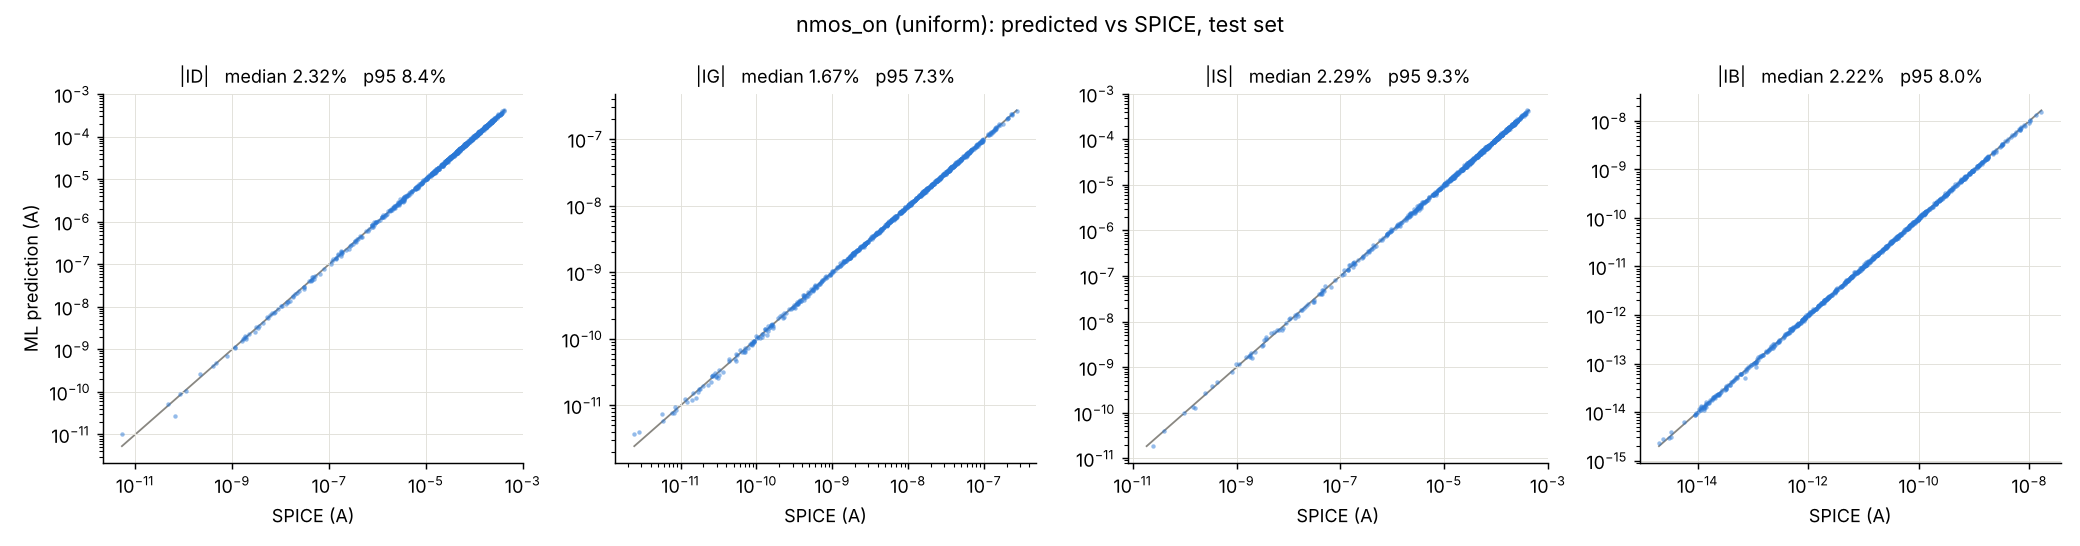
\includegraphics[width=\linewidth]{parity_nmos_on.png}\\[2pt]
\small (a) NMOS ON\\[4pt]
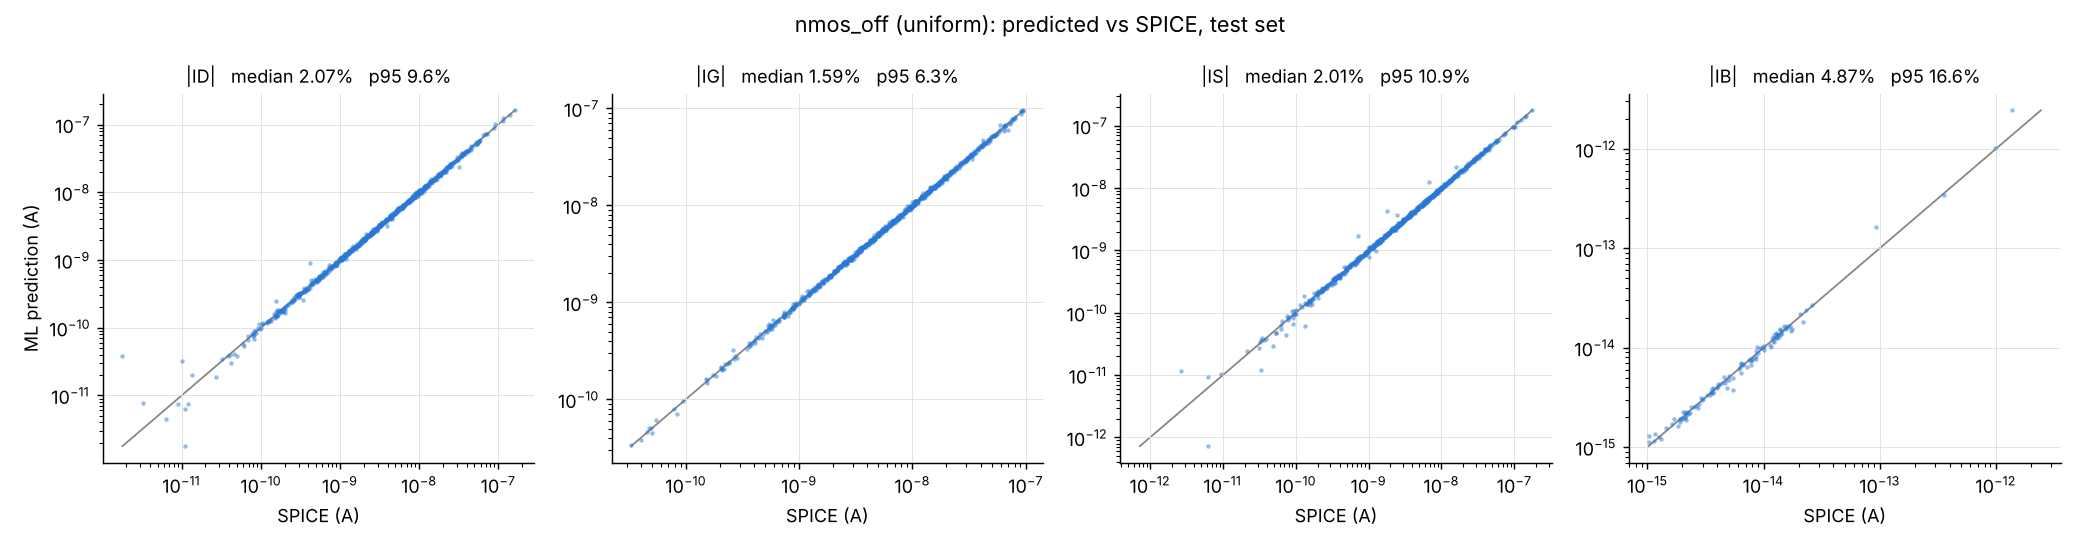
\includegraphics[width=\linewidth]{parity_nmos_off.png}\\[2pt]
\small (b) NMOS OFF\\[4pt]
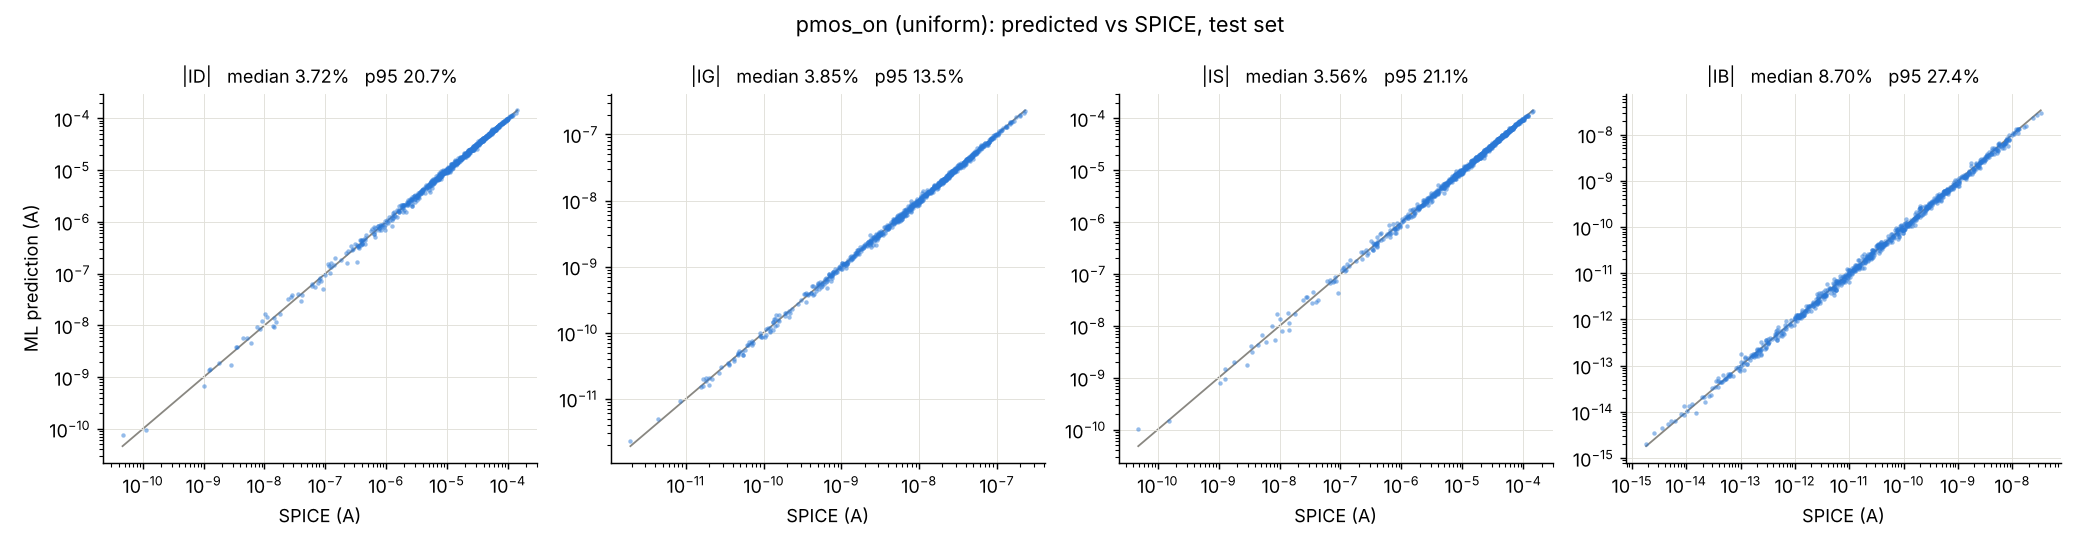
\includegraphics[width=\linewidth]{parity_pmos_on.png}\\[2pt]
\small (c) PMOS ON\\[4pt]
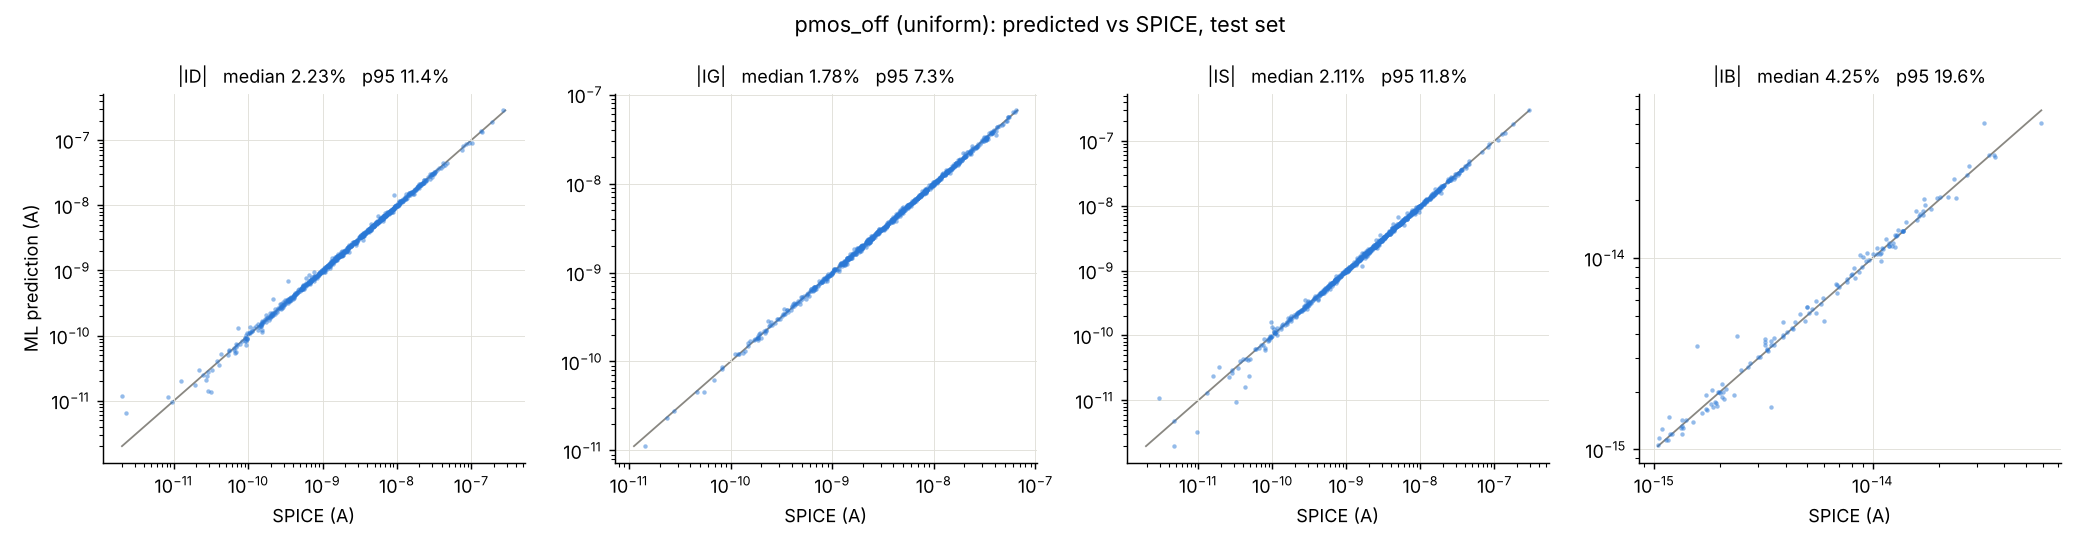
\includegraphics[width=\linewidth]{parity_pmos_off.png}\\[2pt]
\small (d) PMOS OFF
\caption{Predicted vs SPICE currents on the uniform test rows for the chosen
model of each case.}
\label{fig:parity}
\end{figure}

\begin{figure}[H]
\centering
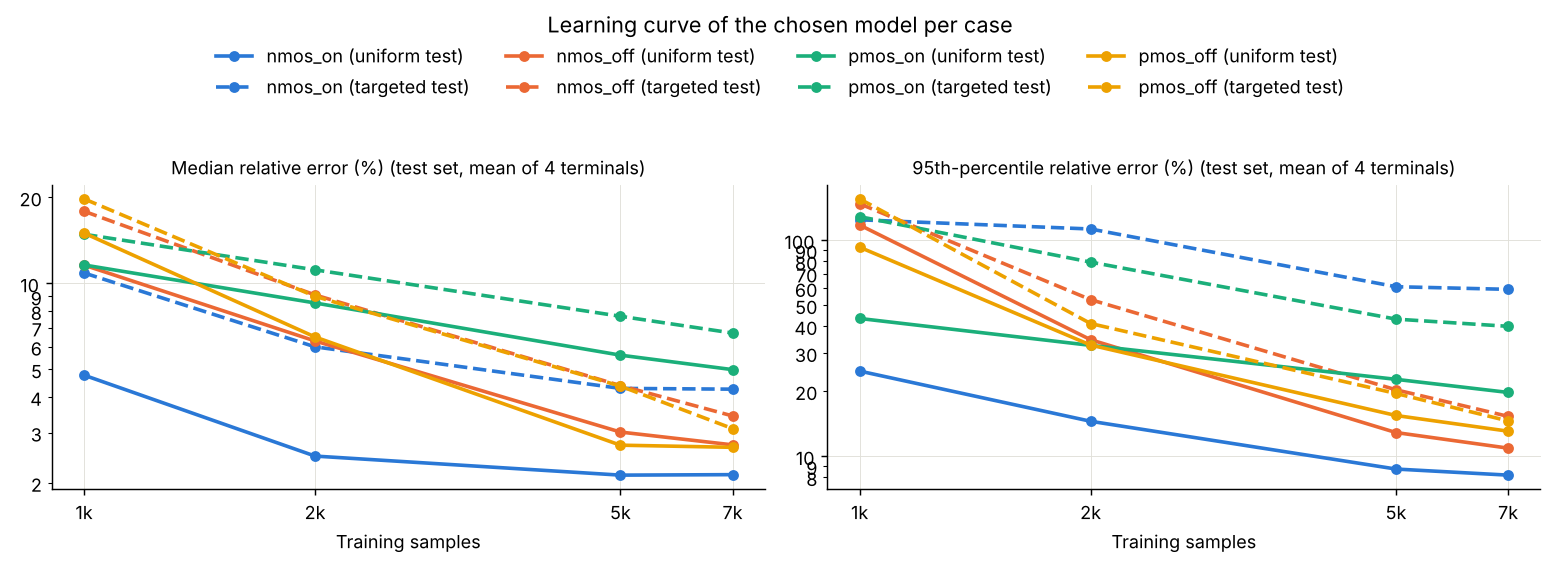
\includegraphics[width=0.85\linewidth]{learning_curve.png}
\caption{Learning curve of the chosen model per case (solid: uniform test
rows; dashed: test rows near gate voltages).}
\label{fig:learning}
\end{figure}

% ==================================================================
\section{Gate-Level Validation}
\label{sec:gates}

\subsection{Aim}

The transistor models predict the currents of a single transistor. This part
checks whether they can also predict the leakage of a complete logic gate.
\begin{itemize}
    \item \textbf{Leakage of a gate:} the DC current it draws from the
          $V_{DD}$ supply while its inputs are held at 0 or $V_{DD}$.
    \item \textbf{Method:} find the leakage with SPICE and with the models,
          then compare the two.
\end{itemize}

\subsection{Gates tested}

We used five static CMOS gates. Every transistor is minimum size,
$W = L = 22$\,nm.

\begin{table}[H]
\centering
\begin{tabular}{lllc}
\toprule
Gate & Transistors & Internal nodes & Input cases \\
\midrule
INV   & 1 PMOS, 1 NMOS                   & none                      & 2 \\
NAND2 & 2 parallel PMOS, 2 series NMOS   & $x$, between the two NMOS & 4 \\
NOR2  & 2 series PMOS, 2 parallel NMOS   & $y$, between the two PMOS & 4 \\
AND2  & NAND2 followed by INV            & $x$ and the NAND2 output  & 4 \\
OR2   & NOR2 followed by INV             & $y$ and the NOR2 output   & 4 \\
\bottomrule
\end{tabular}
\caption{Gates used for the validation: 18 input cases in total.}
\label{tab:gates}
\end{table}

\begin{itemize}
    \item Inputs are written $A$ then $B$: NAND2 \texttt{01} means $A = 0$,
          $B = V_{DD}$.
    \item NAND2 stack: the NMOS driven by $A$ is next to the output, the one
          driven by $B$ is next to ground.
    \item NOR2 stack: the PMOS driven by $A$ is next to $V_{DD}$, the one
          driven by $B$ is next to the output.
\end{itemize}

\subsection{PVT corners}

A corner is one operating condition. We drew 200 corners at random, from the
same ranges as the datasets (Table~\ref{tab:corner}).

\begin{table}[H]
\centering
\begin{tabular}{ll}
\toprule
Part of a corner & Range \\
\midrule
Supply voltage $V_{DD}$ & 0.81 to 0.99\,V \\
Temperature & $-40$ to $125\,^\circ$C \\
vth0, toxe, ndep, u0, xj for all NMOS & nominal $\pm 10\%$ \\
vth0, toxe, ndep, u0, xj for all PMOS & nominal $\pm 10\%$ \\
\bottomrule
\end{tabular}
\caption{Contents of one PVT corner.}
\label{tab:corner}
\end{table}

The same 200 corners are used for every gate, and again for the parity
checker. In total there are $18 \times 200 = 3600$ simulations.

\subsection{SPICE reference}

For every case and corner, a Python script writes a netlist and runs an
\texttt{.op} (DC operating point) analysis in ngspice. The lines below are
from the NAND2 netlist with $A = B = 1$ at corner 0 (model cards left out).
They show the sources and the first transistor; the other three transistors
are written the same way.

\begin{verbatim}
.temp 87.773
vsupply vdd 0 DC 0.842208
vin_a   a   0 DC 0.842208
vin_b   b   0 DC 0.842208
* M<name> d g s b, each terminal through a 0 V source v<name>_<terminal>
mp1 mp1_d mp1_g mp1_s mp1_b pch W=22n L=22n AD=9.68e-16 AS=9.68e-16
vmp1_d out mp1_d DC 0
vmp1_g a   mp1_g DC 0
vmp1_s vdd mp1_s DC 0
vmp1_b vdd mp1_b DC 0
\end{verbatim}

Each transistor terminal is connected to its node through a 0\,V source.
This does not change the circuit, but SPICE reports the current through it.
Each simulation therefore records:
\begin{itemize}
    \item the current delivered by \texttt{vsupply}, which is the reference
          leakage;
    \item the four terminal currents of every transistor;
    \item the voltages of the output and the internal nodes.
\end{itemize}

\subsection{Leakage from the models}

The estimate is made in three steps for each simulation.
\begin{enumerate}
    \item \textbf{Terminal voltages.} Inputs are 0 or $V_{DD}$. The output
          and internal node voltages are taken from the SPICE run, because
          the models predict currents and not voltages.
    \item \textbf{Terminal currents.} A transistor is ON if its gate voltage
          is above $V_{DD}/2$ (NMOS) or below it (PMOS). The model for its
          case predicts $I_d$, $I_g$, $I_s$ and $I_b$.
    \item \textbf{Supply current.} The predicted currents are combined into
          the current drawn from $V_{DD}$ (Section~\ref{sec:combine}).
\end{enumerate}

\subsection{Combining the currents}
\label{sec:combine}

The project statement says to use the predicted currents to calculate the
gate leakage, but it does not give a formula. We used two methods. Both use
only the currents predicted by the models.

\paragraph{Method 1: direct sum.}
The supply current is the sum of the currents into all transistor terminals
connected to $V_{DD}$:
\begin{equation}
I_{VDD} = \sum_{\mathrm{terminals\ at\ } V_{DD}} I_{\mathrm{terminal}}.
\end{equation}
This is the simplest method, but it has a weak point:
\begin{itemize}
    \item the sum contains the source current of every ON PMOS connected to
          $V_{DD}$;
    \item an ON transistor inside a gate has almost no voltage across it, so
          its channel carries only what the OFF transistors let through;
    \item the models predict this small current poorly.
\end{itemize}

\paragraph{Method 2: KCL formula (main result).}
The same sum is used, but the drain and source currents of ON transistors
are never taken from the models. They are replaced using KCL: the currents
into a node add up to zero, and so do the four currents of one transistor
(Table~\ref{tab:used}).

\begin{table}[H]
\centering
\begin{tabular}{lll}
\toprule
Transistor & Method 1 uses & Method 2 uses \\
\midrule
OFF & $I_d$, $I_g$, $I_s$, $I_b$ & $I_d$, $I_g$, $I_s$, $I_b$ \\
ON  & $I_d$, $I_g$, $I_s$, $I_b$ & $I_g$ and $I_b$ only; channel current from KCL \\
\bottomrule
\end{tabular}
\caption{Predicted currents used by the two methods.}
\label{tab:used}
\end{table}

With exact currents the two methods give the same answer. They differ only
because the predicted currents have errors.

\subsection{Example: inverter with input 0}

The PMOS is ON and the NMOS is OFF. The source and body of the PMOS are
connected to $V_{DD}$.

\paragraph{Method 1.}
\begin{equation}
I_{VDD} = I_s^{P} + I_b^{P}.
\end{equation}
This uses the source current of the ON PMOS.

\paragraph{Method 2.}
KCL for the PMOS, and KCL at the output node, give
\begin{equation}
I_s^{P} = -\left(I_d^{P} + I_g^{P} + I_b^{P}\right), \qquad
I_d^{P} + I_d^{N} = 0.
\end{equation}
Putting these into the Method 1 sum:
\begin{equation}
I_{VDD} = I_d^{N} - I_g^{P}.
\end{equation}
The leakage is the drain current of the OFF NMOS plus the gate current
leaving the ON PMOS. The source current of the ON PMOS is no longer needed.
The other gates are handled the same way, with one KCL equation per internal
node.

\subsection{Check of the formulas}

Before using the models, the terminal currents recorded by SPICE were put
through both methods and compared with the supply current from SPICE, in all
3600 simulations.
\begin{itemize}
    \item Method 1 matches within a relative difference of $10^{-15}$.
    \item Method 2 matches within $4.5 \times 10^{-7}$.
    \item Both formulas are therefore correct, and the errors reported below
          come from the models.
\end{itemize}

\subsection{Results}

All results in this section use Method 2. The error of one simulation is
$|I_{ML} - I_{SPICE}| / |I_{SPICE}|$. The bias is the median of
$(I_{ML} - I_{SPICE}) / I_{SPICE}$, so a negative bias means the estimate is
usually too low. Table~\ref{tab:gateoverall} gives the error over all 3600
simulations, Fig.~\ref{fig:gateparity} shows every simulation, and
Table~\ref{tab:gateresults} gives the error of each case.

\begin{table}[H]
\centering
\begin{tabular}{lr}
\toprule
Median error & 1.33\% \\
95th percentile (p95) error & 4.71\% \\
Mean error & 1.81\% (98.2\% mean accuracy) \\
Simulations with error below 5\% & 95.7\% \\
Simulations with error below 10\% & 99.7\% \\
\bottomrule
\end{tabular}
\caption{Error of the gate leakage over all 3600 simulations.}
\label{tab:gateoverall}
\end{table}

\begin{figure}[H]
\centering
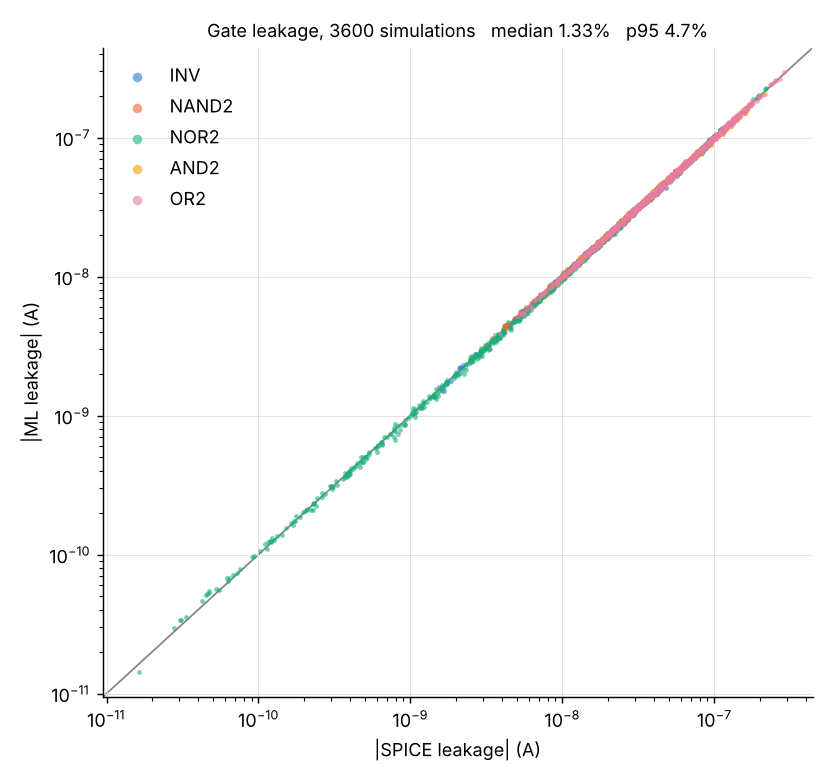
\includegraphics[width=0.45\textwidth]{gate_parity.png}
\caption{Gate leakage from the models against gate leakage from SPICE for
all 3600 simulations. Points on the diagonal line are exact.}
\label{fig:gateparity}
\end{figure}

\begin{table}[H]
\centering\small
\begin{tabular}{lcrrrrrr}
\toprule
     &        & \multicolumn{2}{c}{Median leakage (nA)} & & \multicolumn{3}{c}{Error} \\
\cmidrule(lr){3-4}\cmidrule(lr){6-8}
Gate & Inputs & SPICE & ML & Bias & Median & p95 & Mean \\
\midrule
INV   & 0  & 25.40 & 25.61 & $-0.13\%$ & 1.43\% & 4.16\% & 1.71\% \\
INV   & 1  & 14.53 & 14.44 & $+0.20\%$ & 1.30\% & 5.18\% & 1.74\% \\
\midrule
NAND2 & 00 & 20.54 & 20.47 & $-0.06\%$ & 1.45\% & 5.21\% & 1.81\% \\
NAND2 & 01 & 25.32 & 25.50 & $-0.12\%$ & 1.43\% & 4.16\% & 1.70\% \\
NAND2 & 10 & 18.93 & 18.63 & $-0.94\%$ & 1.70\% & 4.25\% & 1.90\% \\
NAND2 & 11 & 29.00 & 28.82 & $+0.19\%$ & 1.31\% & 5.09\% & 1.73\% \\
\midrule
NOR2  & 00 & 50.51 & 50.79 & $-0.20\%$ & 1.44\% & 4.17\% & 1.74\% \\
NOR2  & 01 & 24.80 & 24.64 & $-0.11\%$ & 1.00\% & 3.64\% & 1.34\% \\
NOR2  & 10 & 8.57  & 8.09  & $-3.04\%$ & 3.26\% & 7.72\% & 3.61\% \\
NOR2  & 11 & 0.74  & 0.74  & $-0.43\%$ & 2.94\% & 9.28\% & 4.50\% \\
\midrule
AND2  & 00 & 51.29 & 51.38 & $+0.10\%$ & 0.85\% & 3.27\% & 1.16\% \\
AND2  & 01 & 56.16 & 55.63 & $+0.04\%$ & 0.88\% & 3.02\% & 1.17\% \\
AND2  & 10 & 48.16 & 47.55 & $-0.27\%$ & 0.91\% & 2.95\% & 1.15\% \\
AND2  & 11 & 58.16 & 57.67 & $-0.29\%$ & 1.13\% & 3.48\% & 1.37\% \\
\midrule
OR2   & 00 & 83.11 & 83.26 & $-0.17\%$ & 1.06\% & 3.47\% & 1.30\% \\
OR2   & 01 & 54.38 & 54.19 & $-0.30\%$ & 1.10\% & 3.50\% & 1.37\% \\
OR2   & 10 & 35.53 & 35.12 & $-1.06\%$ & 1.44\% & 3.67\% & 1.67\% \\
OR2   & 11 & 26.99 & 27.35 & $-0.30\%$ & 1.39\% & 4.10\% & 1.67\% \\
\midrule
All   &    & 30.25 & 30.37 & $-0.28\%$ & 1.33\% & 4.71\% & 1.81\% \\
\bottomrule
\end{tabular}
\caption{Gate results for each case (Method 2). Each row covers the 200
corners.}
\label{tab:gateresults}
\end{table}

\subsection{Where the error is largest and smallest}

\paragraph{Largest: NOR2 \texttt{10} and \texttt{11} (3.3\% and 2.9\% median).}
\begin{itemize}
    \item The PMOS next to $V_{DD}$ is OFF, and its source current is more
          than 99.5\% of the supply current. The estimate depends on this
          one predicted current.
    \item Its drain is at the internal node $y$: 0.15 to 0.20\,$V_{DD}$ in
          case \texttt{10}, and 0.89 to 0.93\,$V_{DD}$ in case \texttt{11}.
    \item Only a few dozen of the 10{,}000 PMOS OFF dataset rows lie in each
          of these regions, so the model is less accurate there.
\end{itemize}

\paragraph{Smallest: AND2 and OR2 (0.9\% and 1.3\% median).}
Their leakage is the sum of two stages, so it does not depend on a single
predicted current.

\subsection{One estimate with the wrong sign}

\begin{table}[H]
\centering
\begin{tabular}{ll}
\toprule
Simulation & NOR2 \texttt{11}, corner 76 ($-38\,^\circ$C) \\
SPICE leakage & $+16$\,pA, the smallest of all 3600 simulations \\
Model estimate & $-14$\,pA \\
Absolute error & 31\,pA \\
\bottomrule
\end{tabular}
\caption{The only simulation where the estimate has the wrong sign.}
\label{tab:sign}
\end{table}

Here the source current of the OFF PMOS is the difference of a channel
current (33\,pA) and a gate current (17\,pA) that almost cancel. In the
other 3599 simulations the largest error is 15.2\%.

\subsection{Comparison of the methods}

Table~\ref{tab:variants} gives the error over all 3600 simulations for every
way of computing the leakage that we used.

\begin{table}[H]
\centering
\begin{tabular}{lrr}
\toprule
Method & Median error & p95 error \\
\midrule
Method 1: direct sum & 3.93\% & 15.7\% \\
Method 2: KCL formula (main result) & 1.33\% & 4.7\% \\
Method 2, inverter gate voltage set to exactly 0 or $V_{DD}$ & 1.41\% & 5.0\% \\
Method 2, also counting current from inputs at $V_{DD}$ & 1.10\% & 3.7\% \\
\bottomrule
\end{tabular}
\caption{Error for each way of computing the gate leakage.}
\label{tab:variants}
\end{table}

\paragraph{Method 1 against Method 2.}
\begin{itemize}
    \item In four cases (INV \texttt{1}, NAND2 \texttt{11}, NOR2 \texttt{10},
          NOR2 \texttt{11}) no ON transistor is connected to $V_{DD}$ by its
          drain or source, so the two methods give the same result.
    \item In the other 14 cases the median error is 2.7\% to 8.0\% with
          Method 1 and 0.8\% to 1.7\% with Method 2.
\end{itemize}

\paragraph{Inverter gate voltage.}
\begin{itemize}
    \item In AND2 and OR2 the inverter is driven by the NAND2 or NOR2
          output, which is up to 1.8\% of $V_{DD}$ away from 0 or $V_{DD}$.
    \item The main result uses this recorded voltage. Setting it to exactly
          0 or $V_{DD}$ gives a slightly higher error.
\end{itemize}

\paragraph{Current from the inputs.}
\begin{itemize}
    \item An input held at $V_{DD}$ also supplies a small gate current. The
          main result counts only the current from the supply.
    \item In the last row this input current is counted as leakage in both
          SPICE and the estimate.
\end{itemize}

% ==================================================================
\section{Circuit-Level Validation: Parity Checker}
\label{sec:circuit}

\subsection{Circuit and evaluation}
This part checks whether the transistor models can estimate the static
leakage of a complete circuit by combining gate predictions. The circuit
checks eight data bits and one even-parity bit:
\begin{equation}
e=d_0\oplus d_1\oplus\cdots\oplus d_7\oplus p.
\end{equation}
Output 0 means valid even parity; output 1 flags an error. A balanced tree
combines the eight data bits, followed by an XOR with $p$. Each XOR uses
four NAND2 gates, giving \textbf{32 NAND2 gates and 128 transistors}.
All transistors use $W=L=22$\,nm and $AD=AS=W(2L)$, matching the
junction-area setup used for the regenerated training data.

All $2^9=512$ input vectors are evaluated at the same 200 PVT corners as
Section~\ref{sec:gates}: \textbf{102,400 circuit cases}. Vector order is
$d_0,\ldots,d_7,p$. The reference is the supply current of the complete
transistor circuit, $I_{\mathrm{SPICE}}=-i(\texttt{vsupply})$, simulated
using a DC input sweep in ngspice-47. Separate primary-input source currents
are excluded from this main leakage definition.

\subsection{Leakage estimation}
For each corner, the four ordered NAND input states form a lookup table
of predicted supply leakage and signed input gate currents: 800 entries
in total. Supply leakage uses the gate-level KCL formula
(Section~\ref{sec:combine}); each input current is the sum of the NMOS and
PMOS gate-terminal currents at that pin. Boolean evaluation selects the
entry for each NAND. Input order is preserved because NAND states
\texttt{01} and \texttt{10} can have different leakage.

\paragraph{Plain gate sum.}
The baseline adds the 32 isolated-gate supply predictions:
\begin{equation}
\widehat I_{\mathrm{plain}}=\sum_{j=1}^{32}\widehat I_{\mathrm{supply},j}.
\end{equation}
In an isolated gate, external sources supply its input currents. In the
complete circuit, another gate supplies the current into an internally
driven high input. The plain sum omits this contribution.

\paragraph{Internal input-current correction.}
Under the ideal-rail approximation, we therefore use
\begin{equation}
\widehat I_{\mathrm{corrected}}=\widehat I_{\mathrm{plain}}+
\sum_{(j,q)\in\mathcal H_{\mathrm{internal}}}\widehat I_{g,jq},
\end{equation}
where $\mathcal H_{\mathrm{internal}}$ contains high receiving pins driven
by other gates. Each pin is counted once, including multiple loads of one
driver. Currents retain their signs, positive into the receiving pin.
Primary-input currents remain excluded; a separate variant includes them
in both prediction and reference.

The circuit estimate uses Boolean logic and the lookup, with no
complete-circuit SPICE voltages as prediction inputs. The lookup does
inherit the isolated-gate SPICE voltages used in Section~\ref{sec:gates}.
The correction accounts for current ownership but does not solve coupled
analog voltages.

\subsection{Validation and results}
The implementation checks all 512 Boolean patterns, the 32-gate/128-transistor
structure, input-current ownership, missing measurements and simulated logic
levels. The saved reference contains every corner--vector pair, and all
recorded NAND outputs agree with Boolean evaluation. The largest output
rail deviation is 0.5366\% of $V_{DD}$; primary inputs deviate by at most
$4.96\times10^{-12}$\,V.

Relative error is $|\widehat I-I_{\mathrm{SPICE}}|/|I_{\mathrm{SPICE}}|$;
bias is the median signed relative error. Table~\ref{tab:circuitresults}
reports percentages over all cases. The diagnostic rows replace ML currents
with isolated-gate SPICE currents while keeping the same aggregation.

\begin{table}[H]
\centering\small
\begin{tabular}{lrrrr}
\toprule
Estimate & Bias (\%) & Median (\%) & p95 (\%) & Mean (\%)\\
\midrule
ML plain sum & $-21.62$ & 21.62 & 54.08 & 24.76\\
ML corrected & $-0.62$ & 1.14 & 3.63 & 1.40\\
ML corrected + primary inputs & $-0.60$ & 1.13 & 3.55 & 1.38\\
SPICE lookup plain & $-21.51$ & 21.51 & 53.85 & 24.61\\
SPICE lookup corrected & $-0.60$ & 0.60 & 1.78 & 0.71\\
\bottomrule
\end{tabular}
\caption{Circuit leakage errors. Only the primary-input variant includes
primary-input source currents in its reference.}
\label{tab:circuitresults}
\end{table}

The corrected estimate gives \textbf{1.14\% median and 1.40\% mean error},
or \textbf{98.60\% mean accuracy}. Median SPICE and corrected ML leakage are
1.1582 and 1.1432\,$\mu$A, respectively; plain ML gives 0.8207\,$\mu$A.
The large improvement over the plain sum shows the importance of counting
internally supplied input currents (Fig.~\ref{fig:circuitparity}).

\begin{figure}[H]
\centering
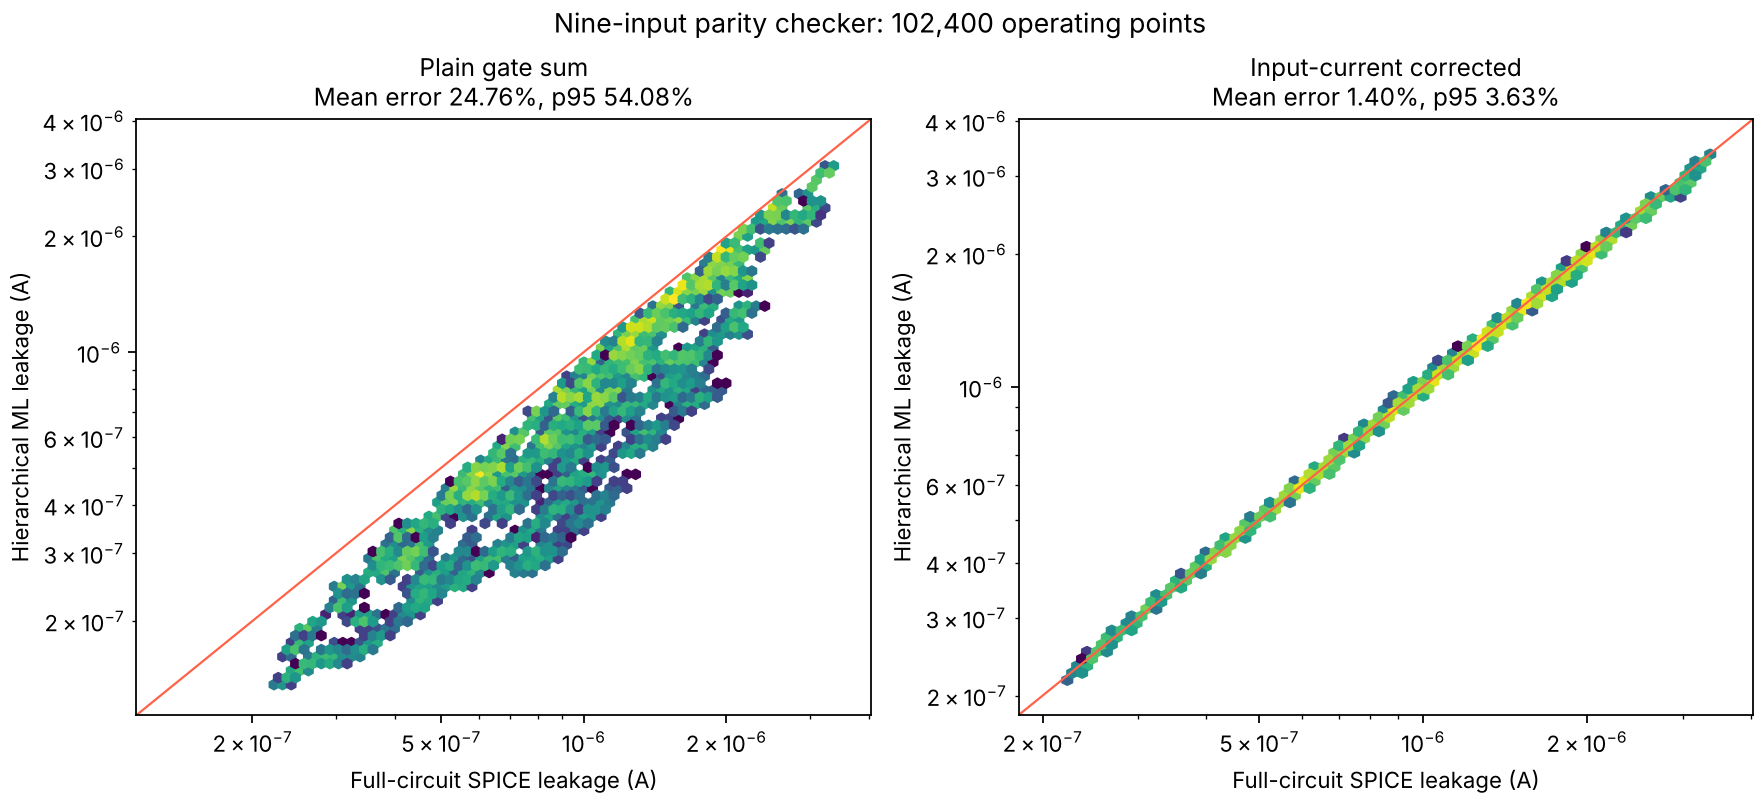
\includegraphics[width=0.85\linewidth]{circuit_parity.png}
\caption{Plain and corrected circuit estimates against SPICE. The diagonal
indicates exact agreement over the 102,400 cases.}
\label{fig:circuitparity}
\end{figure}

\subsection{Worked example and error analysis}
For vector \texttt{000000000} at corner 0 ($V_{DD}=0.842208$\,V,
$T=87.773\,^\circ$C), there are eight NANDs in state \texttt{00}, sixteen
in \texttt{01}, none in \texttt{10}, and eight in \texttt{11}. Thus,
$\widehat I_{\mathrm{plain}}=8\widehat I_{00}+16\widehat I_{01}+8\widehat I_{11}$.
Adding the internal input currents gives
\begin{equation}
\widehat I_{\mathrm{corrected}}=
1.020264+0.207899=1.228163\;\mu\mathrm{A}.
\end{equation}
The full-circuit reference is 1.243591\,$\mu$A, giving 1.2406\% error.

The corrected circuit mean error (1.40\%) is below that of isolated NAND2s
(1.79\%). Summation can average some model errors, although analog loading
introduces additional error. Even the corrected SPICE lookup has 0.71\%
mean error: perfect isolated-gate currents do not make the hierarchical
approximation exact.

The worst case is vector \texttt{111111110}, corner 72, at 0.94936\,V and
$124.91\,^\circ$C. SPICE gives 2.92193\,$\mu$A and ML gives
2.72699\,$\mu$A: \textbf{6.67\% error}. The hottest temperature quartile
has 2.13\% mean error, compared with 0.97--1.28\% in the other quartiles.
Other PVT parameters also vary, so this association does not isolate a
causal temperature effect.

% ==================================================================
\section{Limitations and Improvements}
\label{sec:limits}

\paragraph{Transistor models.}
PMOS ON is the weakest model (5.4\% median test error, against about 3\% for
the other cases), and the OFF body current has the largest errors of any
terminal. The learning curve (Fig.~\ref{fig:learning}) shows the OFF and PMOS
ON models still improving at 7k training rows, so more training data, or an
ensemble of several MLPs, would reduce these errors.

\paragraph{Gates.}
The largest gate errors (NOR2 \texttt{10} and \texttt{11}) come from an OFF
PMOS whose drain sits at an internal-node voltage that few dataset rows
cover. Adding samples at the internal-node voltages of stacked transistors
would target this directly. The model estimate also takes the output and
internal node voltages from SPICE; a fully SPICE-free flow would have to
predict these voltages as well.

\paragraph{Circuit.}
The lookup assumes ideal input rails and isolated-gate operating points.
Fanout and non-ideal node voltages remain unmodelled, in addition to
transistor prediction errors. Analog-input/load-aware gate models or a
coupled voltage solution could improve accuracy; circuit evaluation data
must remain outside training.

\end{document}
